\documentclass[a4paper]{article}

\usepackage{tabularx}
\usepackage[pages=all, color=black, position={current page.south}, placement=bottom, scale=1, opacity=1, vshift=5mm]{background}
\SetBgContents{
	\tt This work is shared under a \href{https://creativecommons.org/licenses/by-sa/4.0/}{CC BY-SA 4.0 license} unless otherwise noted
}      % copyright

\usepackage[margin=1in]{geometry} % full-width

% AMS Packages
\usepackage{amsmath}
\usepackage{amsthm}
\usepackage{amssymb}

% Unicode
\usepackage[utf8]{inputenc}
\usepackage{hyperref}
\hypersetup{
	unicode,
%	colorlinks,
%	breaklinks,
%	urlcolor=cyan, 
%	linkcolor=blue, 
	pdfauthor={Author One, Author Two, Author Three},
	pdftitle={A simple article template},
	pdfsubject={A simple article template},
	pdfkeywords={article, template, simple},
	pdfproducer={LaTeX},
	pdfcreator={pdflatex}
}

% Vietnamese
%\usepackage{vntex}

% Natbib
\usepackage[sort&compress,numbers,square]{natbib}
\bibliographystyle{mplainnat}

% Theorem, Lemma, etc
\theoremstyle{plain}
\newtheorem{theorem}{Theorem}
\newtheorem{corollary}[theorem]{Corollary}
\newtheorem{lemma}[theorem]{Lemma}
\newtheorem{claim}{Claim}[theorem]
\newtheorem{axiom}[theorem]{Axiom}
\newtheorem{conjecture}[theorem]{Conjecture}
\newtheorem{fact}[theorem]{Fact}
\newtheorem{hypothesis}[theorem]{Hypothesis}
\newtheorem{assumption}[theorem]{Assumption}
\newtheorem{proposition}[theorem]{Proposition}
\newtheorem{criterion}[theorem]{Criterion}
\theoremstyle{definition}
\newtheorem{definition}[theorem]{Definition}
\newtheorem{example}[theorem]{Example}
\newtheorem{remark}[theorem]{Remark}
\newtheorem{problem}[theorem]{Problem}
\newtheorem{principle}[theorem]{Principle}

\usepackage{graphicx, color}
%\usepackage{comment}
\graphicspath{{fig/}}

%\usepackage[linesnumbered,ruled,vlined,commentsnumbered]{algorithm2e} % use algorithm2e for typesetting algorithms
\usepackage{algorithm, algpseudocode} % use algorithm and algorithmicx for typesetting algorithms
\usepackage{mathrsfs} % for \mathscr command

\usepackage{lipsum}
\usepackage{subfigure}

% Author info
\title{Comparing the Performance of the $\mathcal{EL}$-Reasoner with the HermiT and ELK Reasoners on the Subsumption Reasoning Task}

\date{
	Vrije Universiteit Amsterdam\\%
	November 23, 2023
}


\begin{document}
	\maketitle

	\begin{abstract}
    This paper introduces the development and utilisation of an ontology tailored for the sushi application domain, alongside the creation of a reasoner based on $\mathcal{EL}$-logic to facilitate reasoning about the knowledge encapsulated in the ontology, specifically for the task of subsumption testing. Subsequently, the self-developed reasoner was tested and compared with two established Description Logics (DL) reasoners, namely HermiT and ELK.
    
    The sushi ontology, constructed in OWL (Web Ontology Language), enables sushi restaurants to intelligently answer specific queries from customers interested in sushi dishes. Additionally, the $\mathcal{EL}$-reasoner was built based on the $\mathcal{EL}$-Completion Algorithm and was used to compute the subsumers of classes represented in the ontology. Ultimately, we compare the performance of reasoning using the self-developed reasoner with two other well-known DL reasoners: HermiT and ELK. HermiT is based on the more expressive Description Logics $\mathcal{ALC}$, whereas ELK is an $\mathcal{EL}$-reasoner optimized for speed. This combination allows for the exploration of the limitations of $\mathcal{EL}$-Description Logics and also allows for comparison against a well-known $\mathcal{EL}$-reasoner. The investigation aims to find out how many subsumed classes could be found in different scenarios and ontologies. 
    
    The results show that our self-developed reasoner, when tested on multiple ontologies of varying size and expressivity, is upper-bounded by the ELK reasoner and the number of found classes differed, on average, within 1 class from the other reasoners. Moreover, the HermiT and ELK reasoners both outperformed the $\mathcal{EL}$-reasoner in terms of reasoning speed. Observations showed that the computational time increased dramatically when the self-developed reasoner was used on large ontologies.\\

		\noindent\textbf{Keywords:} Description Logics, Reasoning, $\mathcal{EL}$-Completion Algorithm, Subsumption, Ontology
	\end{abstract}


    \section{Introduction}
    % include in introduction: background info on knowledge representation, description logics, and ontologies. Research question and hypothesis (+why do we expect this?)
In the realm of computer science, knowledge representation plays a crucial role in structuring and formalizing information in a format that can be understood and manipulated by computational systems. The primary aim of knowledge representation is to capture knowledge about a domain, make it explicit, and enable reasoning and inference. At the heart of knowledge representation lie logics, and in particular, Description Logics (DLs). Description Logics are a family of logic-based knowledge representation languages that have formal semantics \cite{baaderDL}. This family of logics is employed for the structural representation of knowledge within a given application domain and is often used in the field of artificial intelligence. 
Particularly, in recent years, DLs have grown in significance, serving as the formal foundation for the most expressive ontology languages today, such as the OWL (Web Ontology Language) family \cite{rudolph}.

In contrast to the more expressive yet semi-decidable nature of First-Order Logic (FOL), Description Logics (DLs), being a fragment of FOL, offer the advantage of being decidable. This means that there exists an algorithm that can in theory determine the satisfiability, i.e., the truth or falsehood, of any statement in the logic. Besides, DLs allow for efficient reasoning in practical applications. One common reasoning task in DLs is the task of computing subsumption, i.e., sub- and super-class relationships. In subsumption testing, we want to determine whether a concept \textit{C} is subsumed by \textit{D} ($O \models C \sqsubseteq D$), implying that \textit{C} is a subset of \textit{D}. Moreover, DLs form the underpinning logic for the Web Ontology Language (OWL), a standard in the representation of ontologies on the Semantic Web.

This research compares the computation of subsumption relationships using a self-developed reasoner based on the $\mathcal{EL}$-completion algorithm with the two well-known DLs reasoners HermiT and ELK. ELK was selected since, similarly to the self-developed reasoner, it is specialized for the lightweight ontology language OWL $\mathcal{EL}$ and therefore serves as a good benchmark. On the other hand, HermiT was selected to investigate the effect of using a more expressive reasoner on the performance in comparison to the developed $\mathcal{EL}$-reasoner. The reasoners were tested using an OWL ontology that was specifically developed for this research and two existing ontologies that vary in size and expressiveness. The self-developed ontology was tailored for the sushi application domain and developed in Protégé \footnote{https://protege.stanford.edu/}.

The evaluation of DLs reasoners' performance commonly involves metrics such as the level of expressiveness they can support and the reasoning speed. Reasoners with greater expressivity have the capacity to infer additional knowledge from an ontology, allowing them to establish a greater number of subsumption relationships between represented concepts. Nevertheless, this heightened expressivity often accompanies a trade-off in terms of reasoning speed.

\subsection{Research Question and Hypotheses}
To investigate the inferred subsumption-relationships and reasoning speed among the three reasoners, the following research question was set up:

    \begin{quote}
    % MAYBE NEED TO UPDATE IT 
         \textit{Does the self-developed reasoner based on the $\mathcal{EL}$-completion algorithm result in better performance, as measured by the number of subsumed classes and reasoning speed, compared to using the HermiT and ELK reasoners?}

         %How does the performance, defined by the number of subsumed classes and reasoning speed, differ when using the self-developed reasoner based on the $\mathcal{EL}$-completion algorithm in comparison to the HermiT and ELK reasoners?
    \end{quote}

    It is hypothesised that the self-developed $\mathcal{EL}$-reasoner will result in a lower number of subsumers compared to HermiT due to its limited expressivity; $\mathcal{EL}$ cannot handle the concept operators negation ($\neg$), disjunction ($\sqcup$), and the bottom concept ($\bot$) which are used in DLs. In contrast, HermiT is a reasoner based on $\mathcal{ALC}$-logic, which is more expressive than $\mathcal{EL}$-logic. Therefore, it is expected that HermiT will infer more knowledge from an ontology and accordingly more subsumption relationships. On the other hand, we anticipate HermiT to exhibit prolonged reasoning times, as the computational complexity tends to increase for expressive reasoners that support intricate constructs and relationships, resulting in higher computational demands. When comparing our $\mathcal{EL}$-reasoner with the ELK Reasoner, it is anticipated that ELK will have a faster reasoning speed, as it utilizes multi-core and multi-processor systems to speed up the reasoning process. In terms of reasoning, we anticipate that our $\mathcal{EL}$-reasoner can derive approximately as many subsumption relationships as ELK since both support the lightweight ontology language OWL $\mathcal{EL}$.
    
    %This paper describes the development of an ontology in Protégé and the implementation of a Description Logic Reasoner to reason with the ontology and compute the subsumers of all class names in the created ontology. An ontology was developed using Description Logic for an intelligent system designed to support restaurants specializing in sushi. The ontology aims to provide a structured representation of various sushi dishes, encompassing their ingredients, properties of these ingredients, and relationships, enabling intelligent responses to customer queries related to preferred ingredients and dietary requirements. The ontology was created following the menu of the restaurant "ILoveSushi Amsterdam". Due to the size and variety of dishes on this menu, a hierarchy was made to simplify the ontology and to remove dishes and other products that fall outside of this project's scope. 
    
    \section{The Sushi Ontology}
    \label{sec:intro}
    An ontology was developed using DLs for an intelligent system designed to support restaurants specializing in sushi. The ontology aims to provide a structured representation of various sushi dishes, encompassing their ingredients, properties of these ingredients, and relationships, enabling intelligent responses to customer queries related to preferred ingredients and dietary requirements. The ontology was created following the menu of the restaurant "ILoveSushi Amsterdam". Due to the size and variety of dishes on this menu, a hierarchy was made to simplify the ontology and to remove dishes and other products that fall outside of this project's scope.  

    \subsection{Ontology hierarchy}
    The ontology follows a straightforward hierarchy with three main subclasses: \textit{Food}, \textit{IngredientCharacteristic} and \textit{Country}. The \textit{Food} subclass encompasses the subclasses \textit{Sushi}, and \textit{SushiIngredients}. \textit{Sushi} is further subdivided into multiple subclasses based on their cooking styles, roll type, spiciness, the number of ingredients the sushi contains, and dietary requirements such as vegetarian and non-vegetarian. An important subclass of \textit{Sushi} is \textit{NamedSushi}, which is composed of \textit{Maki}, \textit{Nigiri} and \textit{Sashimi} and represents sushi that can be found on the menu.
    
    To formalise sushi that contains only vegetarian ingredients, the class \textit{VegetarianSushi} was defined. A vegetarian sushi is a sushi that contains only vegetarian ingredients, which is defined by the \textit{VegetarianIngredient} class. In addition, to formalize the specific ingredients that the different sushi types can contain, ingredients were defined in the \textit{SushiIngredient} class. Ingredients are classified based on certain defining properties, such as \textit{Fish}, \textit{Grain}, and \textit{Vegetable}.

    The \textit{IngredientCharacteristic} class encompasses classes for the cooking style of a dish and classes for different spiciness levels. This enables the formalization of sushi into types that are, for example, raw and hot. Ultimately, the \textit{Country} subclass encompasses entities representing different countries of origin. These countries utilize data properties to assert their names in a string format. This class was introduced since certain rolls, such as the California roll, have a particular place of origin (e.g. Japan or America). To better illustrate the hierarchy and the sub-superclass relationships, the most important classes of the ontology are defined below:
    \newline
    \newline

    % thought a hierarchy with short explanation would be more clear than the text above. Still need to finish it. O
    \begin{itemize}
        \item \textbf{Food}:
        \begin{itemize}
            \item \textbf{Sushi}: Represents a sushi. \textit{Sushi} contains multiple subclasses based on their cooking styles, roll type, the number of ingredients the sushi contains, spiciness, and dietary requirements such as vegetarian and non-vegetarian ingredients.
            \begin{itemize}
                \item \textbf{VegetarianSushi}: represents sushi that contains only vegetarian ingredients, as defined by the \textit{VegetarianIngredient} class.
                \item \textbf{NonVegetarianSushi}: represents sushi that does not only contain vegetarian ingredients. Defined as: NonVegetarianSushi $\equiv$ Sushi and (not (VegetarianSushi)).
                \item \textbf{SimpleSushi}: represents sushi that contains at most three ingredients.
                \item \textbf{InterestingSushi}: represents sushi that contains at least five ingredients.
                \item \textbf{SpicySushi}: represents sushi that contains a spicy ingredient. 
                \item \textbf{RealJapaneseSushi}: represents sushi dishes that are of Japanese origin.
                \item \textbf{NamedSushi}: represents sushi that can be found on the menu. Contains the subclasses \textit{Maki}, \textit{Nigiri}, and \textit{Sashimi}.
            \end{itemize}
            \item \textbf{SushiIngredient}: this represents the various ingredients that a sushi can contain. Some of the subclasses of \textit{SushiIngredient} include \textit{Fish}, \textit{Vegetable} and \textit{VegetarianIngredient}.
        \end{itemize}
        \item \textbf{IngredientCharacteristic}: represents the characteristic of a sushi ingredient and contains the subclasses \textit{Spiciness} and \textit{CookingStyle}.
        \begin{itemize}
            \item \textbf{Spiciness}: represent the spiciness level of an ingredient. Can be either hot, medium or mild.
            \item \textbf{CookingStyle}: represents the cooking style of \textit{Fish} or \textit{Meat}. Can be either \textit{Raw} or \textit{Cooked}.
        \end{itemize}
    \end{itemize}
    
    \begin{figure}[hbt]
        \centering
        \subfigure[]{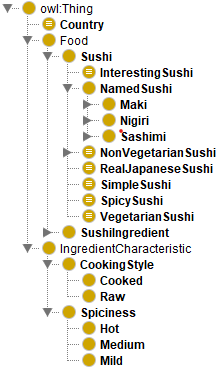
\includegraphics[width=0.28\textwidth]{hierarchyMain.png}}
        \subfigure[]{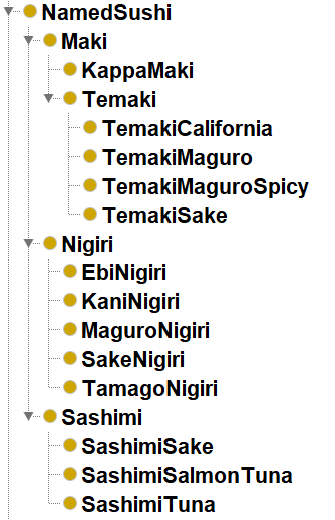
\includegraphics{hierarchy2.png}}
        \caption{Sushi ontology hierarchy in Protégé with (a) the main classes where \textit{NamedSushi} is collapsed and (b) subclasses of the \textit{NamedSushi} class.}
        \label{fig:hierarchies}
    \end{figure}

    \subsubsection{Object properties}
    Object properties are binary predicates that relate concepts in an ontology. The relations between classes in the Sushi Ontology are represented using the following object properties, with \textit{hasIngredient} and \textit{hasCharacteristic} being the most important object properties in our ontology:

        \begin{itemize}
        \item \textbf{hasIngredient}: specifies that \textit{Food} has an ingredient \textit{SushiIngredient}. Has the domain \textit{Food} and range \textit{SushiIngredient}.
        \item \textbf{isIngredientOf}: defines that \textit{SushiIngredient} is an ingredient of \textit{Sushi}. Inverse of \textit{hasIngredient}.
        \item \textbf{hasCountryOfOrigin}: defines the country of origin of a dish.
        \item \textbf{hasCharacteristic}: defines that \textit{SushiIngredient} has the characteristic \textit{IngredientCharacteristic}, which can be either the spiciness level or cooking style.
        \begin{itemize}
            \item \textbf{hasCookingStyle}: specifies that \textit{Fish} and \textit{Meat} can have the cooking style \textit{Cooked} or \textit{Raw}. The domain is \textit{Fish} and \textit{Meat} and the range is \textit{CookingStyle}. Sub-property of \textit{{hasCharacteristic}}.
            \item \textbf{hasSpiciness}: relates ingredient to a spiciness level, which can be either hot, medium, or mild. The range is \textit{Spiciness}.
        \end{itemize}
    \end{itemize}

	\subsection{Axioms and Inferences}
Closure axioms were used to represent subclass (i.e., $\sqsubseteq$) and equivalence (i.e., $\equiv$) relationships between concepts in the ontology. They were used for all named sushis to ensure the closure of the open-world assumption of the ontology. Most sushi dishes are defined by closure axioms in combination with existential restrictions, such as in the example below. These axioms represent "EbiNigiri has the ingredients prawn and rice and no other".\\

\begin{quote}
    \textit{EbiNigiri $\sqsubseteq$ hasIngredient only (Prawn or Rice)}\\
    \textit{EbiNigiri $\sqsubseteq$ hasIngredient some Prawn}\\
    \textit{EbiNigiri $\sqsubseteq$ hasIngredient some Rice} \\
\end{quote}

Besides, when running a reasoner, some inferred class relationships were obtained. For example, the definition of \textit{VegetarianSushi}, as shown below, inferred that KappaMaki was a vegetarian sushi as it contains the ingredients cucumber, nori seaweed, and rice, which are all defined as vegetarian ingredients in the ontology.

\begin{quote}
    \textit{VegetarianSushi $\equiv$ Sushi and (hasIngredient only VegetarianIngredient)}\\
    \textit{VegetarianIngredient $\equiv$ SushiIngredient and (Egg or Fruit or Grain or NoriSeaweed or Sauce or Vegetable)}
\end{quote}

    
 Moreover, specific sushi types that contained at least five ingredients were inferred as interesting sushi, whereas types with at most three ingredients were inferred as simple sushi. We formalised this using a number restriction on the number of outgoing role connections for \textit{hasIngredient}. As an example. the equivalence axiom for InterestingSushi, as shown below, was used to infer all sushi types that were regarded as interesting sushi. For example, \textit{TemakiCalifornia} is inferred as interesting sushi in our ontology since \textit{TemakiCalifornia} has the ingredients avocado, cucumber, crab, and tobiko, \textit{TemakiCalifornia} is a subclass of \textit{Temaki} and \textit{Maki}, and \textit{Maki} has the ingredients rice and nori seaweed. Therefore, it has at least 5 ingredients and is inferred as interesting sushi.

    \begin{quote}
        \textit{InterestingSushi $\equiv$ Sushi and (hasIngredient min 5 owl:Thing)}\\
        \textit{SimpleSushi $\equiv$ Sushi and (hasIngredient max 3 owl:Thing)}
    \end{quote}

Axioms were also used to impart nominal restrictions to dishes based on their origin countries. Country entities, on the other hand, use the data property \textit{hasName} for string-based naming schemes (the class \textit{UnitedStates} for example has the name \textit{"United States of America"}). The class \textit{RealJapaneseSushi} was formalized as follows:\\
    \begin{quote}
        \textit{RealJapaneseSushi $\equiv$ Sushi and (hasOriginCountry value Japan)}
    \end{quote}
	
	\section{$\mathcal{EL}$-Reasoner}
     The developed reasoner to derive subsumption relationships between concepts from the ontologies is based on the $\mathcal{EL}$-Completion Algorithm. Reasoning in $\mathcal{EL}$ allows the concept operators top ($\top$), conjunction ($\sqcap$), and existential restrictions ($\exists$). However, the limited expressivity of $\mathcal{EL}$ does lead to some limitations, such as not being able to handle negations ($\neg$), the bottom concept ($\bot$), and value restrictions ($\forall$). As a result, contradictions cannot be expressed in DL $\mathcal{EL}$. For testing subsumption in $\mathcal{EL}$, it has been demonstrated that reasoning can be performed in polynomial time \cite{Brandt}. 


%E.g. make the algorithm faster and test on the ontologies provided. See if we now get more inferences. Thus your implementation will not always be able to infer all the subsumers for any given class. In your report you should also mention how you deal with concepts/axioms that are not supported by your reasoner.
%The value restrictor is not present in EL

    \subsection{$\mathcal{EL}$-Completion Algorithm}
    % describe the rules and the algorithm in the report. Since I only showed a pseudo code algorithm in the lecture, there must have been some things in the implementation you decided on - what data structures you used, which loops, how you determined whether to apply a rule.

    % Check if this first sentence is correct
    The $\mathcal{EL}$-reasoner tests subsumption by applying rules and determining whether a concept \textit{C} is subsumed by another concept \textit{D} with respect to a given ontology $\mathcal{O}$, denoted as $O \vDash C \sqsubseteq D$. This implies that \textit{C} (i.e., the subclass) is at least as general as \textit{D} (i.e. the superclass), or in other words, every instance of \textit{C} is also an instance of \textit{D}.
    
    In essence, the $\mathcal{EL}$-completion algorithm determines whether $O \vDash C \sqsubseteq D$. The algorithm iteratively constructs a special model of $\mathcal{O}$ with an element $d \in \mathbb{C}^I$. In this model, $d$ satisfies all concepts $D'$ for which $\mathcal{O}\models C \sqsubseteq D'$. The algorithm initiates with a single element $d_0$ to which the initial concept \textit{C} is assigned. Throughout the algorithm, concepts are assigned to elements and special rules are applied towards satisfying those concepts. If \textit{D} eventually gets assigned to $d_0$, we conclude that $O \vDash C \sqsubseteq D$. The rules that are used in the algorithm are shown in Table \ref{ELrules}.

\begin{table}[ht]
    \centering
    \caption{$\mathcal{EL}$-Completion Rules}
    \begin{tabular}{|l|p{0.7\textwidth}|}
        \hline
        $\top$-rule & Add $\top$ to any individual. \\
        \hline
        $\sqcap$-rule 1 & If $d$ has $C \sqcap D$ assigned, assign also $C$ and $D$ to $d$. \\
        \hline
        $\sqcap$-rule 2 & If $d$ has $C$ and $D$ assigned, assign also $C \sqcap D$ to $d$. \\
        \hline
        $\exists$-rule 1 & If $d$ has $\exists r.C$ assigned:
                           \begin{enumerate}
                               \item If there is an element $e$ with the initial concept $C$ assigned, make $e$ the $r$-successor of $d$.
                               \item Otherwise, add a new $r$-successor to $d$, and assign to it as the initial concept $C$.
                           \end{enumerate} \\
        \hline
        $\exists$-rule 2 & If $d$ has an $r$-successor with $C$ assigned, add $\exists r.C$ to $d$. \\
        \hline
        $\sqsubseteq$-rule & If $d$ has $C$ assigned and $C \sqsubseteq D \in T$, then also assign $D$ to $d$. \\
        \hline
    \end{tabular}
    \label{ELrules}
\end{table}

    \subsection{Implementation of the $\mathcal{EL}$-Subsumption Algorithm}
    
    \subsubsection{Dealing with axioms and concept outside of $\mathcal{EL}$ logic}
    
    When running the $\mathcal{EL}$-reasoner, firstly, all equivalence axioms in the TBox are converted to general concept inclusions (GCIs), since $\mathcal{EL}$ assumes no equivalence axioms in the TBox. Consequently, equivalence axioms of the form C $\equiv$ D were replaced by the subsumption axioms C $\sqsubseteq$ D and D $\sqsubseteq$ C.

    To deal with axioms not supported by $\mathcal{EL}$ such as the \textit{Disjoint} axiom we simply delete them from the TBox because we cannot make any use of them inside of the $\mathcal{EL}$ domain. Once the equivalence axioms are converted, we deal only with general concept inclusions (GCIs).
    On the other hand, we decided to retain all the concept types that are not supported by $\mathcal{EL}$, such as the value restriction, but just not apply the rules related to them. This could still let us infer some concepts that would not be inferred if we removed all the ones outside of $\mathcal{EL}$.

    \subsubsection{Data structures used}

    To implement the graph for the $\mathcal{EL}$-completion algorithm we have built a custom graph class, along with a node and relation class specialized for this reasoning task. The structure underneath it is a dictionary, where the keys are the nodes names, generated with an incremental id, and the values are the node classes. These contain the successor relations along with the predecessor relations. The first helps us optimize the application of the first existential rule, restricting the search between all the edges of the graph,  while the latter helps us optimize the search for the second existential rule.

    As we will see, our implementation relies on data structures that memorize the newly generated nodes, edges, or concepts. For that we decided to use sets since they are safer for this task and we do not have to do any search operations on them.

    \subsubsection{The subsumption algorithm in detail}
    We decided to implement the algorithm in a way that applies the rules only between newly created nodes, concepts or edges and all the other items we already have in our graph. We optimized the reasoning task pruning all the rules that we have already applied in between older nodes.
    This is done using three data structures one per each type of addition to the graph. These are initialized with the new items at the end of each iteration and will be used on the next one, as can be seen in the pseudocode of Algorithm \ref{alg:your_alg}.

    

    \begin{algorithm}
    \caption{Pseudocode of our $\mathcal{EL}$-Completion Algorithm}
    \label{alg:your_alg}
    \begin{algorithmic}[1] % The number tells where the line numbering should start
    \Procedure{FindSubsumers}{$C0, D0s, t box$}
        \State $\textit{newNodes, newConcepts} \gets \text{Node(initialConcept = C0)}$
            
        
        \While{$\text{newNodes} \neq \emptyset \textbf{ or } \text{newConcepts} \neq \emptyset \textbf{ or } \text{newEdges} \neq \emptyset$}
        
            \For{$node \textbf{ in } newNodes$} % For-in loop
                \State $\textit{nextNewConcepts} \gets \text{ApplyTopRule(node)}$
            \EndFor
            \For{$concept \textbf{ in } newConcepts$} % For-in loop
                \State $\textit{nextNewConcepts, nextNewNodes, nextNewEdges} \gets \text{applyConjunctionAndExistential1(concept)}$
                \State $\textit{nextNewConcepts} \gets \text{applyExistentialRule2(concept)}$
            \EndFor
            \For{$edge \textbf{ in } newEdges$} % For-in loop
                \State $\textit{nextNewConcepts} \gets \text{applyExistentialRule2(edge)}$
            \EndFor
            \State $\textit{newNodes, newConcepts, newEdges} \gets \text{nextNewNodes, nextNewConcepts, nextNewEdges}$
        \EndWhile
        \For{$concept \textbf{ in } initialNode.concepts$} % For-in loop
            \If{$concept \textbf{ in } D0s$}
                \State $\textit{subsumers} \gets \text{concept}$
            \EndIf
        \EndFor
        \State \textbf{return} $\textit{subsumers}$
    \EndProcedure
    \end{algorithmic}
    \end{algorithm}

    The \textit{newConcepts} set is filled with the newly added concepts paired with the respective node on which they have just been added on. This way the \textit{applyConjunctionAndExistential1} and \textit{applyExistential2} functions have enough context to apply the respective rules.
    
    Finally, the  $\top$-rule is exclusively applied to newly created nodes, for trivial reasons, while the second existential rule is the only one applied to new edges, because it is the sole one which could update the graph when a new edge is added.
    

    \section{HermiT and ELK Reasoners}
    %\textcolor{red}{CHECK SECTION ON HERMIT; I FOUND IT HARD TO DESCRIBE IT CLEARLY AND UNDERSTAND HOW THE REASONER EXACTLY WORKS}.

    \subsection{HermiT Reasoner}
    HermiT is a DLs reasoner that employs the novel "hypertableau" calculus and was used as the first reasoner for the comparison with the self-developed $\mathcal{EL}$-Reasoner \footnote[1]{http://www.hermit-reasoner.com/}. Tableaux methods describe systems in which satisfiability is tested by deriving a sequence of ABoxes (tableaux) where each ABox is obtained through inference rules applied on the prior ABox \cite{Horrocks2012TheHO}. This method can be applied to DLs including the more expressive $\mathcal{ALC}$, which allows a broader range of constructors including universal quantification ($\forall$), existential quantification ($\exists$), conjunction ($\sqcap$), disjunction ($\sqcup$), and negation ($\neg$). Moreover, HermiT addresses the challenge of evaluating a great number of potential models and the considerable size of models generated by traditional tableaux reasoners, thereby improving reasoning efficiency \cite{Hermit}. The "hypertableau" calculus decreases the number of possible models that need to be evaluated. Besides, the use of the "anywhere blocking" strategy and other optimization techniques limit the size of the models produced.

    The tableaux method as employed by the HermiT reasoner transforms the main reasoning tasks including subsumption testing into consistency testing by negating the subsumption relationship. This means that to test subsumption, i.e., to decide whether $O \models C \sqsubseteq D$, we check $C \sqcap \neg D$. If it is shown that $C \sqcap \neg D$ is unsatisfiable, we can conclude that $O \models C \sqsubseteq D$.
    
    An OWL ontology $\mathcal{O}$ is commonly composed of property axioms, class axioms, and facts, corresponding to the RBox ($\mathcal{R}$), TBox ($\mathcal{T}$), and ABox ($\mathcal{A}$), respectively. These constitute the knowledge base $\mathcal{K}$ = ($\mathcal{R}$, $\mathcal{T}$, $\mathcal{A}$). To determine whether the knowledge base $\mathcal{K}$ is satisfiable, the tableaux method first normalizes the knowledge base by transforming it into negation normal form (NNF). For computing subsumption relationships between concepts, the tableaux method reduces the reasoning task to satisfiability testing. This means that to test subsumption, i.e., to decide whether $O \models C \sqsubseteq D$, we check whether $C \sqcap \neg D$ is satisfiable. To determine this, the tableaux algorithm generates a sequence of ABoxes, where each $A_i$ is obtained by applying one of the inference rules as shown in Table \ref{TableauxRules}. If no more inference rule can be executed or $A_n$ contains a contradiction, the algorithm terminates. We can conclude that $O \models C \sqsubseteq D$ if it is shown that $C \sqcap \neg D$ is unsatisfiable.

\begin{table}[h]
  \centering
  \caption{Tableaux Method - $\mathcal{ALC}$ Expansion Rules}
  \begin{tabular}{|>{\raggedright\arraybackslash}p{0.25\linewidth}|p{0.7\linewidth}|}
    \hline
    $\sqcap$-rule & $a : C \sqcap D \Rightarrow a : C$, $a : D$ \\
    \hline
    $\sqcup$-rule & $a : C \sqcup D$ and we have neither $a : C$ nor $a : D$ $\Rightarrow a : C$ or $a : D$ \\
    \hline
    $\exists$-rule & $a : \exists r.C$, no $\langle a, b \rangle : r$ s.t. $b : C$ $\Rightarrow \langle a, b \rangle : r$, $b : C$ for a new individual $b$ \\
    \hline
    $\forall$-rule & $a : \forall r.C$, $\langle a, b \rangle : r$ $\Rightarrow b : C$ \\
    \hline
    $T$-rule & $\top \sqsubseteq C \in T$ $\Rightarrow a : C$ for any individual $a$ we already introduced \\
    \hline
  \end{tabular}
  \label{TableauxRules}
\end{table}

    \subsection{ELK Reasoner}
    % CHECK: in slides it says that ELK is used for ELH, but 
    ELK is the second reasoner that was used for comparison with our self-developed $\mathcal{EL}$-Reasoner. This open-source reasoner is a dedicated reasoner designed for the lightweight ontology language OWL $\mathcal{EL}$. ELK distinguishes itself from other OWL $\mathcal{EL}$ reasoning systems by applying inferences in parallel, enabling the method to leverage the capabilities of multiple cores and processors for a faster reasoning process and effectively deal with large ontologies \cite{kazakov}. Furthermore, ELK strategically applies inference rules, eliminating redundant inferences without sacrificing completeness. Coupled with additional implementation techniques, including indexing and efficient join computation, these improvements contribute to a substantial performance boost compared to other $\mathcal{EL}$ reasoners.

    The ELK reasoning component derives consequences of ontological axioms using inference rules. The reasoning process for subsumption testing involves several steps, including indexing, saturation, and taxonomy construction \cite{kazakov}. As it goes beyond the scope of this research, the inference rules and detailed reasoning processes used by ELK are left out.
          
    \section{Methods}
    To compare the self-developed $\mathcal{EL}$-Reasoner with the two open-source reasoners HermiT and ELK, the number of found subsumers and the reasoning speed were analysed. These metrics together define the performance of the reasoners in this research, as the number of found subsumers indicates the level of expressiveness of the reasoner, while the reasoning speed is a measure to test the efficiency of the reasoner. The Sushi ontology was built in the open-source OWL ontology editor and framework Protégé. Besides, two additional open-source ontologies were used which vary in size and expressivity. Given an ontology, the number of subsumers for each class was computed. The reasoning speed was measured by the time it takes to compute the subsumers of each class. The following open-source ontologies were used in addition to the Sushi ontology:

    \begin{itemize}
        \item \textbf{amino-acid.amino-acid-ontology.2.owl}: large ontology representing amino acids. The ontology contains axioms that use existential restrictions ($\exists$, universal quantification ($\forall$), disjunctions ($\sqcup$), and negation ($\neg$).
        \item \textbf{doid.human-disease-ontology.589.owl}: a standardized ontology for human diseases. The ontology contains a large number of classes with sub-superclass relationships but lacks general concept inclusions ($\sqsubseteq$) and equivalence axioms ($\equiv$). 
    \end{itemize}

    \section{Results}
    % To evaluate the performance of the reasoner using the EL-Completion algorithm to a baseline, a comparison was made with the HermiT Reasoner. Here, performance is defined in terms of the number of subsumers that are computed for a given class name. HermiT is a publicly available OWL reasoner based on a novel "hypertableau" calculus. This indicates that HermiT employs an advanced form of tableau reasoning, involving the construction of a tree-like structure, to perform automated reasoning on ontologies expressed in the OWL. Consequently, this research investigates the following research question:

    %Change to testing against HermiT AND Elk
    %Sources for reasoners being optimized
    
    As previously mentioned, this research investigates whether the reasoner implemented, using the $\mathcal{EL}$-completion algorithm, can identify a comparable number of subsumption relationships between classes of a set of ontologies with respect to the popular reasoners HermiT and ELK, in a comparable amount of time. The test procedure consists of one run per ontology over the Sushi ontology and the ontologies mentioned in Section 5. On each run, we test a different reasoner and we compute the number of subsumers per class, along with the time spent by the algorithm to terminate. Subsequently, we isolate randomly 10 classes with a minimum number of subsumers. Finally, we draw two bar plots per ontology: one comparing the time taken to find the subsumers of each class and one comparing the number of subsumers found.

    The bar charts in Figure \ref{fig:sushi} illustrate the results that were obtained for the Sushi ontology.
    \begin{figure}[h!]
        \centering
        \subfigure[]{
            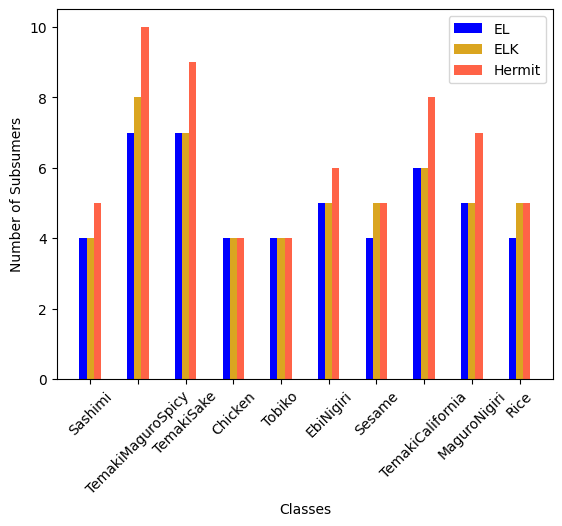
\includegraphics[width=0.45\textwidth]{sushi_subsumers_2.png}
        }
        \hspace{5mm} % Adjust the horizontal space between the figures
        \subfigure[]{
            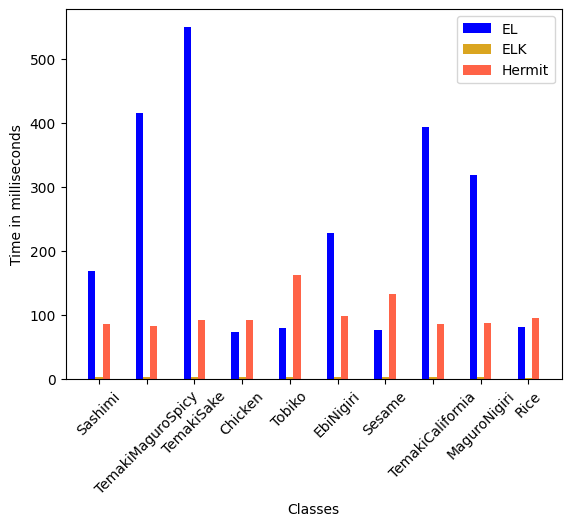
\includegraphics[width=0.45\textwidth]{sushi_time_2.png}
        }
        \caption{Bar plot of the number of subsumers found for the given class (a) and the time taken to compute them (b), considering the sushi ontology.}
        \label{fig:sushi}
    \end{figure}

    In Figure \ref{fig:sushi} we can see that the number of subsumers found by the three reasoners are comparable, differing in one subsumer on average. We can ascertain that the upper bound of the reasoning capabilities of our algorithm are the ones of ELK, given that it implements all the $\mathcal{EL}$ rules with the addition of the bottom rule. In turn, the upper bound of the number of subsumers found by ELK is the one of HermiT, which can trivially be explained by the fact that it exploits all the rules of the $\mathcal{ALC}$ logic.

    Moving to a knowledge base containing over a hundred more axioms (315) but fewer classes (46), we can observe the same results for the amino acids ontology in Figure \ref{fig:amino-acids}. The plot reveals that ELK and HermiT outperform the $\mathcal{EL}$-reasoner in terms of the number of computed subsumers for a given class.
    
    \begin{figure}[h!]
        \centering
        \subfigure[]{
            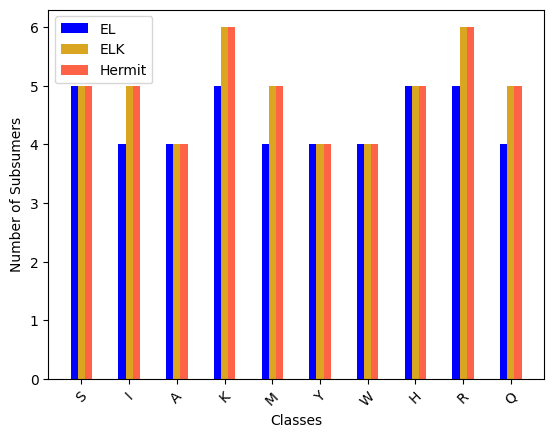
\includegraphics[width=0.45\textwidth]{amino_subsumers_1.png}
        }
        \hspace{5mm} % Adjust the horizontal space between the figures
        \subfigure[]{
            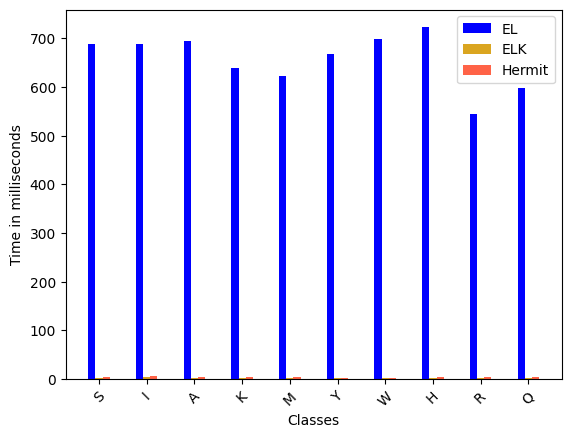
\includegraphics[width=0.45\textwidth]{amino_time_1.png}
        }
        \caption{Bar plot of the number of subsumers found for the given classes (a) and the time taken to compute them (b), considering the amino acids ontology.}
        \label{fig:amino-acids}
    \end{figure}
    We can see that the computing time of our reasoner is starting to scale with the increase of the ontology's dimensions.
    We see this effect at its extreme with the analysis of the reasoner on the human diseases ontology, as shown in Figure \ref{fig:human-diseases}(b).
    In fact, the human diseases ontology counts 16.693 axioms, that have challenged our reasoner. This is also the reason why we computed the subsumers for only 15 classes over the 8.236 it contains, given that it was taking around 10 seconds per class as we can see in Figure \ref{fig:human-diseases}.

    Despite the computation time that, on the other end, doesn't seem to be affected consistently for ELK and Hermit, the number of subsumers found puts all the reasoners in agreement. This proves that our reasoner is still resilient to these ontology dimensions. This agreement is given by the fact that the human diseases ontology contains almost only \textit{subClassOf} axioms, and does not exploit capabilities beyond $\mathcal{EL}$ logic.
    
    \begin{figure}[h!]
        \centering
        \subfigure[]{
            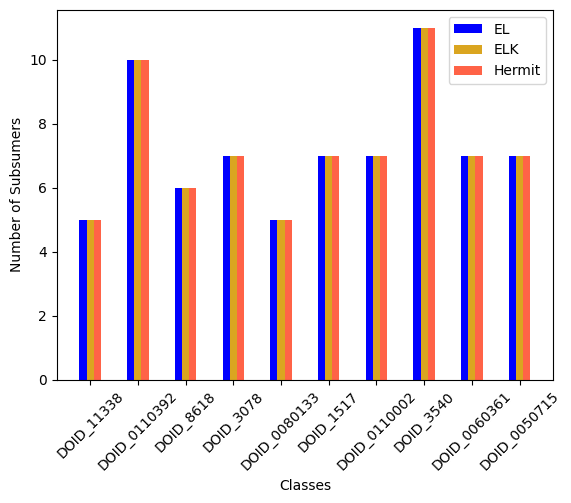
\includegraphics[width=0.45\textwidth]{diseases_subsumers_1.png}
            \label{fig:sushi_subsumers}
        }
        \hspace{5mm} % Adjust the horizontal space between the figures
        \subfigure[]{
            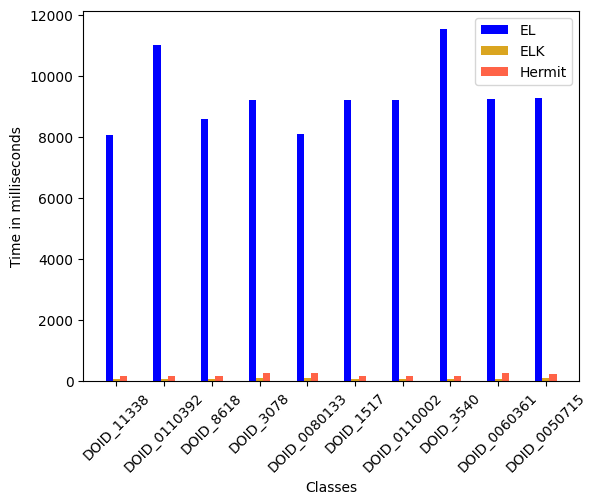
\includegraphics[width=0.45\textwidth]{diseases_time_1.png}
            \label{fig:sushi_time}
        }
        \caption{Bar plot of the number of subsumers found for the given classes (a) and the time taken to compute them (b), considering the human diseases ontology.}
        \label{fig:human-diseases}
    \end{figure}
    

     
    



 \section{Discussion and Conclusion}
 This research investigated whether the self-developed reasoner based on the $\mathcal{EL}$-completion algorithm results in better performance, as measured by the number of subsumed classes and reasoning speed, compared to the HermiT and ELK reasoners. 
 
 %It was hypothesized that the HermiT reasoner could compute more subsumed classes compared to the $\mathcal{EL}$-reasoner while having a longer reasoning speed, given that HermiT supports the more expressive $\mathcal{ALC}$-logic. Besides, it was anticipated that ELK results in comparable results in terms of the number of subsumers that can be found, while having a faster reasoning speed. 

Our findings confirm our hypothesis that our self-developed reasoner is outperformed by the HermiT reasoner and closely matches the ELK reasoner in terms of the number of subsumed classes that could be found. It was revealed that the number of subsumed classes found by the self-developed $\mathcal{EL}$-reasoner is upper-bounded by the ELK reasoner. Besides this result and regardless of ontology size, the reasoner also seemed to be quite robust as the number of found subsumers would, on average, differ by one.

As for speed, it was hypothesized that our reasoner would exhibit longer reasoning time than the ELK reasoner, whereas the HermiT reasoner would exhibit prolonged reasoning time due to its expanded expressiveness. Our observations confirmed the first statement, which was enforced by our reasoner not being optimized for speed and efficiency. We also observed dramatic increases in computational time when our reasoner was used on large ontologies. On the other hand, HermiT outperformed our own reasoner in all tests which is a testament to the efficiency of its "hypertableu" method. In conclusion, this suggests that the $\mathcal{EL}$-reasoner is only suitable for smaller ontologies lest some optimizations were to be made.

 A natural progression of this work involves expanding the capabilities of the $\mathcal{EL}$-reasoner to accommodate greater expressivity. This extension could encompass features such as handling the bottom concept ($\bot$), supporting existential restrictions ($\mathcal{\forall}$), or incorporating role inclusion axioms. Additionally, addressing the observed higher computational time for determining the number of subsumers in the $\mathcal{EL}$-reasoner suggests a need for future research aimed at enhancing the efficiency of the $\mathcal{EL}$-completion algorithm implementation. Nevertheless, despite this computational challenge, the present study has successfully developed a reasoner capable of identifying a comparable number of subsumers when compared to well-established counterparts like HermiT and ELK. Notably, this reasoner offers valuable insights into subsumption relationships between concepts of ontologies.
 



%	\newpage
	\bibliography{refs}
	
	\appendix
	

		
\end{document}